% --- Template for thesis / report with tktltiki2 class ---
% 
% last updated 2013/02/15 for tkltiki2 v1.02

\documentclass[12pt,finnish]{tktltiki2}

% tktltiki2 automatically loads babel, so you can simply
% give the language parameter (e.g. finnish, swedish, english, british) as
% a parameter for the class: \documentclass[finnish]{tktltiki2}.
% The information on title and abstract is generated automatically depending on
% the language, see below if you need to change any of these manually.
% 
% Class options:
% - grading                 -- Print labels for grading information on the front page.
% - disablelastpagecounter  -- Disables the automatic generation of page number information
%                              in the abstract. See also \numberofpagesinformation{} command below.
%
% The class also respects the following options of article class:
%   10pt, 11pt, 12pt, final, draft, oneside, twoside,
%   openright, openany, onecolumn, twocolumn, leqno, fleqn
%
% The default font size is 11pt. The paper size used is A4, other sizes are not supported.
%
% rubber: module pdftex

% --- General packages ---
\usepackage[dvips]{graphicx}
\usepackage[utf8]{inputenc}
\usepackage[T1]{fontenc}
\usepackage{lmodern}
\usepackage{microtype}
\usepackage{amsfonts,amsmath,amssymb,amsthm,booktabs,color,enumitem,graphicx}
\usepackage[pdftex,hidelinks]{hyperref}
\usepackage{setspace}

\onehalfspacing

% Automatically set the PDF metadata fields
\makeatletter
\AtBeginDocument{\hypersetup{pdftitle = {\@title}, pdfauthor = {\@author}}}
\makeatother

% --- Language-related settings ---
%
% these should be modified according to your language

% babelbib for non-english bibliography using bibtex
\usepackage[fixlanguage]{babelbib}
\selectbiblanguage{finnish}

% add bibliography to the table of contents
\usepackage[nottoc]{tocbibind}
% tocbibind renames the bibliography, use the following to change it back
\settocbibname{Lähteet}

% --- Theorem environment definitions ---

\newtheorem{lau}{Lause}
\newtheorem{lem}[lau]{Lemma}
\newtheorem{kor}[lau]{Korollaari}

\theoremstyle{definition}
\newtheorem{maar}[lau]{Määritelmä}
\newtheorem{ong}{Ongelma}
\newtheorem{alg}[lau]{Algoritmi}
\newtheorem{esim}[lau]{Esimerkki}

\theoremstyle{remark}
\newtheorem*{huom}{Huomautus}


% --- tktltiki2 options ---
%
% The following commands define the information used to generate title and
% abstract pages. The following entries should be always specified:

\title{Yhteistoiminnalliset ja sisältöpohjaiset suosittelujärjestelmät}
\author{Johanna Wahtera}
\date{\today}
\level{Kandidaatintutkielma}
\abstract{Aineessa tutustutaan sekä sisältöpohjaiseen että yhteistoiminnalliseen suodattamiseen perustuvien suosittelujärjestelmien toimintaan yleisellä tasolla. Aineesta selviää, mikä on näiden kahden suosittelujärjestelmätyypin oleellisin ero.
Kummastakin järjestelmätyypistä esitellään esimerkki, joka on sisältöpohjaisen suosittelun tapauksessa Flickr-kuvapalvelun tunnisteiden suosittelu käyttäjille. Yhteistoiminnallista suosittelua avataan esittelemällä Netflix Prize -kilpailuun osallistuneen joukkueen suosittelujärjestelmää.}

% The following can be used to specify keywords and classification of the paper:

\keywords{suosittelujärjestelmät, yhteistoiminnallinen suodatus, sisältöpohjainen järjestelmä, Flickr, Netflix}

% classification according to ACM Computing Classification System (http://www.acm.org/about/class/)
% This is probably mostly relevant for computer scientists
% uncomment the following; contents of \classification will be printed under the abstract with a title
 %"ACM Computing Classification System (CCS):"
 \classification{Information systems ->  Information retrieval ->  Retrieval tasks and goals ->  Recommender systems}

% If the automatic page number counting is not working as desired in your case,
% uncomment the following to manually set the number of pages displayed in the abstract page:
%
%% \numberofpagesinformation{16 sivua + 10 sivua liitteissä}
%
% If you are not a computer scientist, you will want to uncomment the following by hand and specify
% your department, faculty and subject by hand:
%
 \faculty{Matemaattis-luonnontieteellinen}
 \department{Tietojenkäsittelytieteen laitos}
 \subject{Tietojenkäsittelytiede}
%
% If you are not from the University of Helsinki, then you will most likely want to set these also:
%
 \university{Helsingin yliopisto}
 \universitylong{HELSINGIN YLIOPISTO --- HELSINGFORS UNIVERSITET --- UNIVERSITY OF HELSINKI} % displayed on the top of the abstract page
 \city{Helsinki}
%


\begin{document}

% --- Front matter ---

\frontmatter      % roman page numbering for front matter

\maketitle        % title page
\makeabstract     % abstract page

\tableofcontents  % table of contents

% --- Main matter ---

\mainmatter       % clear page, start arabic page numbering


\section{Johdanto}
         Internet koostuu valtavasta määrästä monimuotoista sisältöä. Verkkoa selaava käyttäjä löytää niin tuotteita, artikkeleita kuin sivustoja lähes loputtomasti. Rajattomien mahdollisuuksien edessä käyttäjän voi kuitenkin olla vaikeaa löytää jotakin juuri häntä kiinnostavaa. Suuren verkkokaupan laajaa valikoimaa ei voida asettaa kerralla käyttäjän näkyville samalla tavoin kuin perinteisessä kivijalkakaupassa. Sama haaste tulee vastaan kaikenlaisia tuotteita, kuten musiikkia, elokuvia tai artikkeleita selatessa. Hakukoneet ratkaisevat ongelman osittain löytämällä suuresta määrästä tietoa juuri sen, mitä käyttäjä etsii. On kuitenkin tapauksia, joissa käyttäjä ei \textit{tiedä} mitä hän haluaa löytää. On syntynyt tarve henkilökohtaisille kulutussuosituksille.
        
Suosittelujärjestelmä valikoi käyttäjän puolesta tuotteita, joita tarjotaan hänelle kulutettavaksi. Järjestelmä kerää dataa käyttäjästä ja/tai tarjolla olevista tuotteista ja muodostaa datan perusteella suosituksia tuotteista, joita käyttäjä todennäköisesti pitäisi kiinnostavana.

Suosittelujärjestelmän toteutustavat voidaan jakaa kahteen laajempaan ryhmään: sisältöpohjaisiin (content-based) ja yhteistoiminnallisen suodattamisen (collaborative filtering) järjestelmiin. Tässä aineessa keskitymme näiden järjestelmien eroihin ja tutustumme muutamaan esimerkkijärjestelmään.

        Sisältöpohjaisissa järjestelmissä kerätään tietoa palvelun tuotteista ja vertaillaan näitä toisiinsa. Käyttäjälle suositellaan uusia tuotteita sen perusteella, minkälaisia tuotteita hän on menneisyydessä selannut tai hankkinut. Tuotteen merkittävät piirteet kartoitetaan tuoteprofiiliin ja profiilia verrataan toisen tuotteen profiiliin. Tavoitteena on löytää mahdollisimman samankaltaisia profiileja. Tuote voi olla tässä yhteydessä mitä vain käyttäjälle suositeltavaa sisältöä, kuten elokuva tai uutisartikkeli. Elokuvan tapauksessa tuoteprofiiliin merkittäisiin esimerkiksi elokuvan näyttelijät, ohjaaja, valmistusvuosi ja lajityyppi. 
        
        Yhteistoiminnallisen suodattamisen järjestelmät keskittyvät yksittäisen käyttäjän ja tuotteiden ominaisuuksien lisäksi käyttäjäyhteisön välisiin relaatioihin. Käyttäjät lajitellaan samankaltaisiksi heidän antamiensa arvosteluiden perusteella. Samanlaisista asioista pitävät käyttäjät muodostavat oman aliryhmänsä koko käyttäjäyhteisöstä. Tuotteiden samankaltaisuus määritellään vertailemalla useamman samankaltaisen käyttäjän arvosteluja.
        
        Sekä yhteistoiminnalliseen suodattamiseen perustuvat että sisältöpohjaiset suosittelujärjestelmät vaativat toimiakseen tietoa käyttäjän mieltymyksistä. Käyttäjien mielipiteitä kerätään usein suoraan arvosteluiden kautta, mutta toisinaan preferenssit päätellään käyttäjän käyttäytymisestä muin keinoin, kuten esimerkiksi klikkaushistorian perusteella \cite{Das:2007:GNP:1242572.1242610}.
        
\section{Sisältöpohjaiset järjestelmät}
        
\subsection{Yleisesti}

Sisältöpohjaisissa suosittelujärjestelmissä vertaillaan käyttäjälle tarjottavan sisällön ominaisuuksia toisiinsa ja pyritään löytämään niiden väliset samankaltaisuudet.
Jokaiselle tuotteelle muodostetaan tuoteprofiili, johon kerätään tuotteen tärkeimmät ominaisuudet. Nämä tiedot ovat yleensä saatavilla suoraan tekstinä tuotteen tiedoista~\cite{Ullman}.

Profiilien samankaltaisuus määräytyy pitkälti sen perusteella, kuinka paljon samoja luokituksia ja oleellisia sanoja niissä esiintyy. Eräs tähän soveltuvista menetelmistä on Jaccardin kerroin (Jaccard coefficient tai Jaccard index) johon palataan seuraavassa kappaleessa.

Tuoteprofiilin lisäksi myös käyttäjästä rakennetaan käyttäjäprofiili. Käyttäjäprofiili rakentuu samoista osista kuin tuoteprofiili, mutta tuotetiedon paikalle merkitään käyttäjän mieltymys kyseisen tiedon suhteen. Esimerkki tällaisesta tiedosta voisi olla vaikkapa elokuvan lajityyppi, jolloin toiminnasta pitävän käyttäjän profiiliin merkitään lajityypin kohdalle "toiminta".

Joidenkin tuotteiden ominaisuuksia on vaikea vertailla keskenään. Esimerkiksi kuvista on mahdollista saada vain rajallinen määrä suositusjärjestelmän kannalta oleellista tietoa. Tällaisissa tapauksissa järjestelmässä onkin usein käytössä tuotteiden tunnistetoiminto (tags), jossa tuotteiden ominaisuuksia merkitään sanallisin tunnuksin.

Kun vastuu merkitsemisestä on käyttäjällä, voivat tunnisteet jäädä epäselviksi ja niiden määrä vaihdella suurestikin. Käyttäjien välillä ei myöskään välttämättä vallitse yhtenevä mielipide oikeanlaisesta tunnistetyylistä. Kaksi eri käyttäjää saattaakin merkitä samanlaisen kuvan täysin toisistaan poikkeavilla tunnisteilla. Ratkaisua tähän ongelmaan käydään seuraavassa kappaleessa, joka toimii myös esimerkkinä sisältöpohjaisesta suosittelujärjestelmästä.


\subsection{Tunnisteiden suosittelu käyttäjille yhteisötiedon perusteella}

Sigurbjörnsson ja van Zwol~\cite{Sigurbjornsson:2008:FTR:1367497.1367542} esittelevät eri tapoja suositella käyttäjälle tunnisteita, jotka sopivat hänen palveluun lataamaansa sisältöön. Suosittelulla tunnisteista saadaan järjestelmällisempiä ja yhdenmukaisempia.

Käyttäjien motivaatio merkitä kuvansa tunnisteilla tuntuu olevan niiden kyvyssä tuoda heidän lataamansa sisältö paremmin muiden käyttäjien näkyville~\cite{Ames:2007:WWT:1240624.1240772}. Johdonmukaisilla tunnisteilla merkittyihin tuotteisiin törmää palvelua selatessa helpommin kuin sellaisiin, joita ei ole merkitty lainkaan tai jotka on merkitty epäselvästi. Esimerkiksi kuvien kohdalla käyttäjä voi lisätä tunnisteiksi kuvauspaikan ja mitä kuva hänen mielestään esittää. Näiden käyttäjän kirjoittamien tunnisteiden ja kaikkien kuvapalvelusta kerättyjen tunnistetietojen perusteella voidaan kuvaan ehdottaa yleisiä lisätunnisteita. Suositeltujen tunnisteiden käyttö lisää tunnistetyylin johdonmukaisuutta ja helpottaa tietynlaisten kuvien hakua ja suosittelua.

Flickr-kuvapalvelu koostui vuonna 2008 8,5 miljoonasta rekisteröityneestä käyttäjästä ja valtavasta kuvamäärästä. Sigurbjörnsson ja van Zwol tarkastelivat tästä datasta satunnaisesti koostettua 52 miljoonan kuvan osajoukkoa~\cite{Sigurbjornsson:2008:FTR:1367497.1367542}. Jokaisessa kuvassa oli vähintään yksi tunniste. Yhteensä tunnisteita oli noin 188 miljoonaa, joista 3,7 miljoonaa olivat uniikkeja.

	Vain kerran esiintyvät tunnisteet ovat yleensä niin erikoislaatuisia tai kirjoitusvirheellisiä, ettei niitä kannata suositella. Jos taas tunniste on yksi yleisimmin käytetyistä, esimerkiksi vuosiluku, on se yleensä liian geneerinen suositeltavaksi~\cite{Sigurbjornsson:2008:FTR:1367497.1367542}.
	
Käyttäjien antamien tunnisteiden määrä vaihtelee yksilökohtaisesti ja vaikuttaa suosittelun kannattavuuteen. Enimmillään tarkasteltavan joukon käyttäjät olivat merkinneet kuvaan yli 50 tunnistetta. Tällaisissa tilanteissa on vaikeaa tarjota hyödyllisiä tunnistesuosituksia. 64 \% kuvista oli merkitty 1-3 tunnisteella, jolloin suosituksia on helppo muodostaa ja järkevää tarjota.

Tunnisteet voidaan jakaa eri kategorioihin käsittelyn helpottamiseksi. Aineiston suosituimpia tunnistetyyppejä olivat paikat (28 \%), esineet tai artefaktit (16 \%), ihmiset tai ryhmät (13 \%), toiminnot tai tapahtumat (9 \%) ja ajankohdat (7 \%). Loput 27 \% eivät menneet minkään näiden kategorian alle. Ne voitiin kuitenkin luokitella omiin alikategorioihinsa WordNet -kategorisoinnin (WordNet broad categories) avulla.

Tunnisteiden samassa yhteydessä esiintymisten (tag co-occurence) laskeminen on suosittelun ydin. Menetelmä toimii luotettavasti vain suuren datamäärän kanssa, mutta käsiteltävästä aineistosta koostettu alijoukko oli tässä tapauksessa riittävä. Kuten edellä jo käsiteltiin, ovat eri tunnisteet suosittelun kannalta eriarvoisia keskenään. Pelkkä tunnisteiden yhteisesiintymisten laskeminen ei ota huomioon tunnisteiden esiintymisyleisyyttä, joten on suositeltavaa normalisoida tulos tunnisteiden kokonaisesiintymisellä. Normalisointiin esitellään kaksi tapaa: symmetrinen ja epäsymmetrinen.

Symmetrisessä normalisoinnissa voidaan normalisoida kahden tunnisteen $t_{i}$ ja $t_{j}$ yhteiset esiintymiset Jaccardin kertoimen (Jaccard coefficient)
\begin{displaymath}
J (t_{i}, t_{j}):= \frac{|K(t_{i}) \cap K(t_{j})|} {|K(t_{i}) \cup K(t_{j})|}
\end{displaymath}
mukaan, jossa K(t) = \{kuva | kuvalla tunniste t\}.

Jaccardin kerrointa käytetään yleisesti kahden objektin tai joukon samanlaisuuksien mittaamiseen. Sen kaltaiset symmetriset mittaukset soveltuvat hyvin kahden tunnisteen merkitysten vertailuun.

Epäsymmetrisessä normalisoinnissa normalisointi tehdään yhden tunnisteen esiintymismäärän perusteella. Voimme laskea kahden tunnisteen $t_{i}$ ja $t_{j}$ yhteisesiintymisten todennäköisyyden ja normalisoida tuloksen tunnisteen $t_{i}$ esiintymisyleisyydellä 
\begin{displaymath}
P (t_{j} | t_{i}):= \frac{|K(t_{i}) \cap K(t_{j})|} {|K(t_{i})|}
\end{displaymath}
mukaisesti. Tässä P kertoo, millä todennäköisyydellä kuvassa, joka on merkitty tunnisteella $t_{i}$, on myös tunniste $t_{j}$.

Symmetrinen normalisointi tuottaa tunnisteelle hyvin samankaltaisia tunnistesuosituksia~\cite{Sigurbjornsson:2008:FTR:1367497.1367542}. Esimerkiksi tunnisteen \textit{Eiffel Tower} tapauksessa suurimman yhteisesiintymisluvun saavat sanat \textit{Tour Eiffel, Eiffel, Seine, La Tour Eiffel} ja \textit{Paris}. Epäsymmetrisellä mittauksella saman sanan tulokset ovat \textit{Paris, France, Tour Eiffel, Eiffel} ja \textit{Europe}. Nähdään, että epäsymmetrisellä yhteisesiintymisellä löydetään monipuolisempia suositeltavia tunnisteita.

\begin{figure}[]
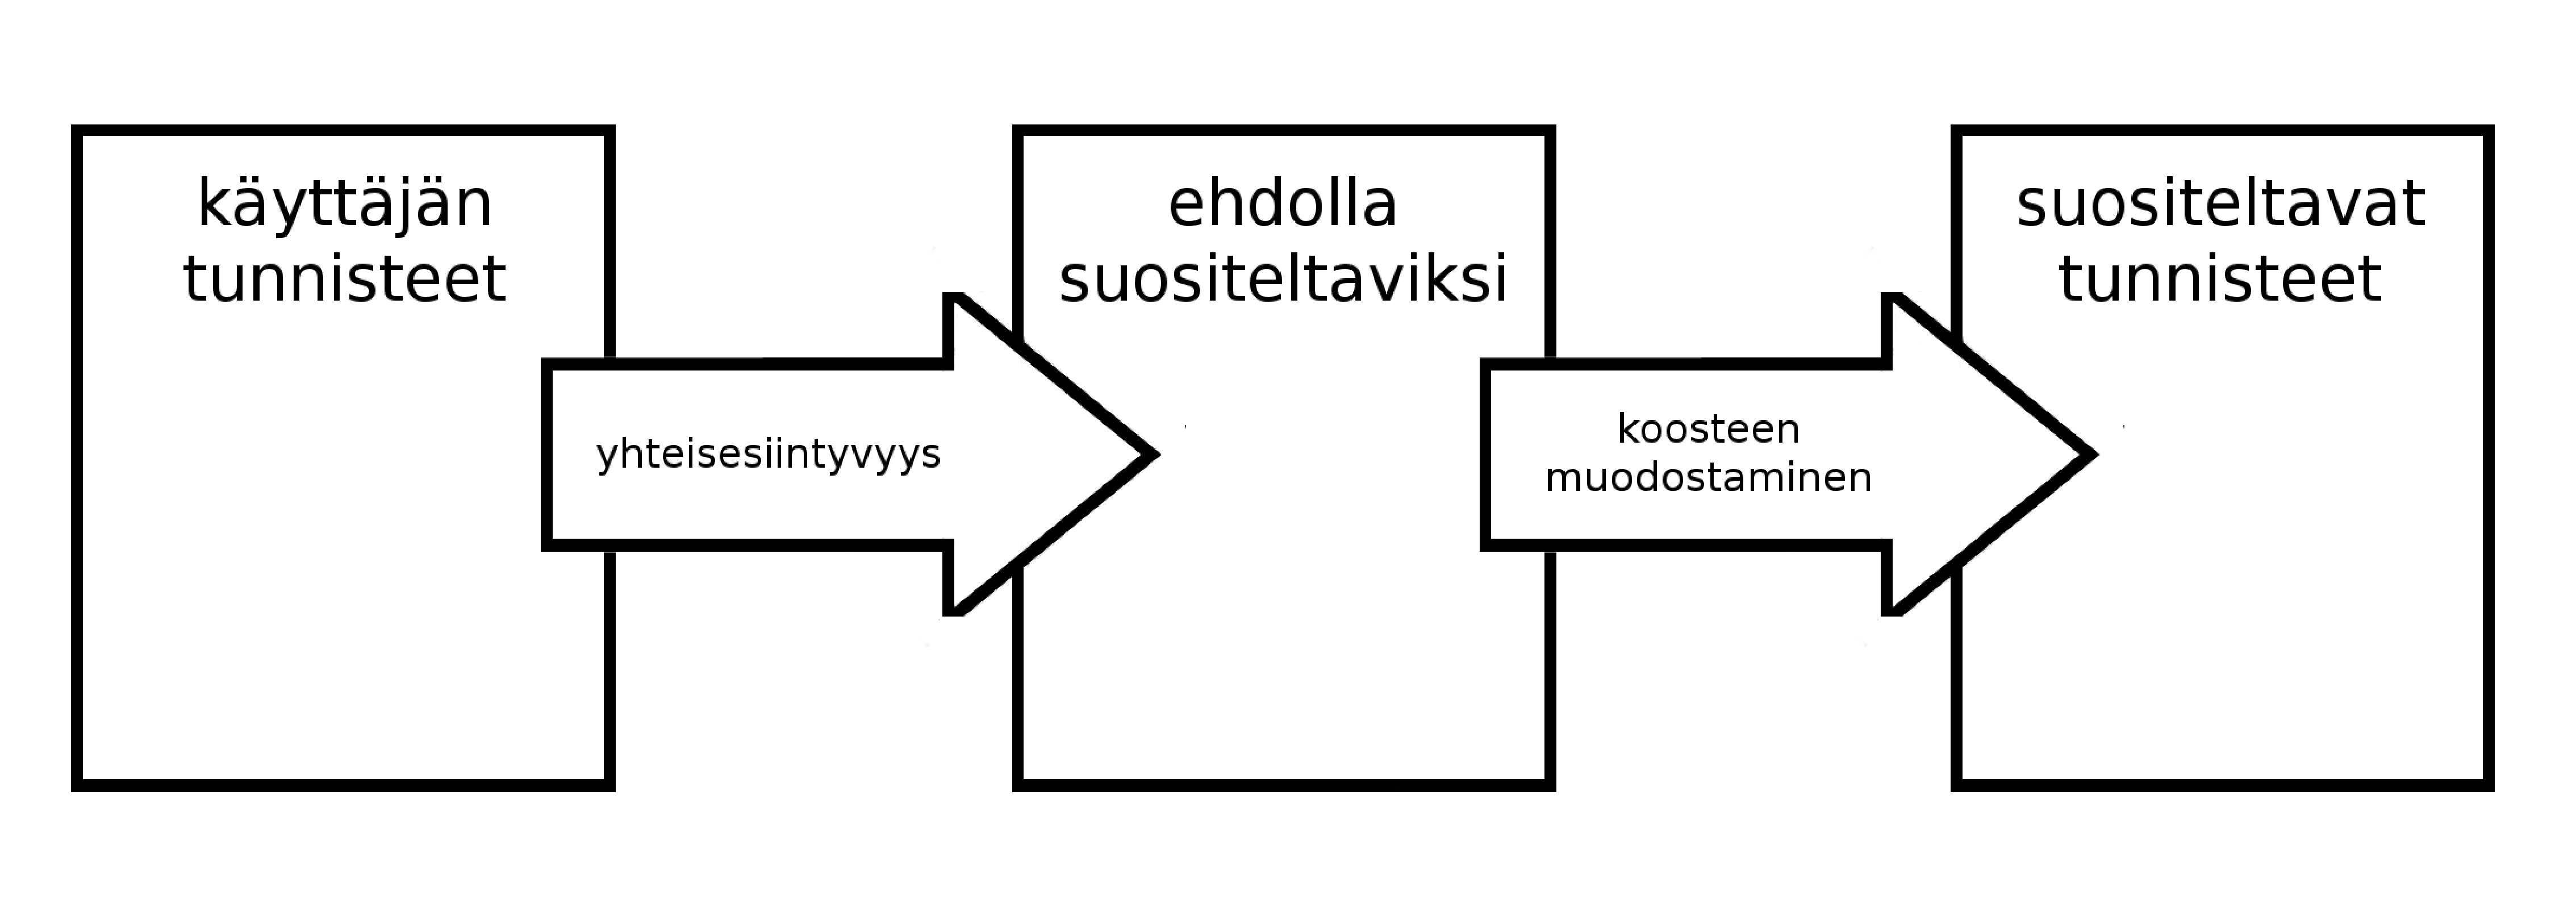
\includegraphics[width = 420pt]{tunnisteidensuosittelu.eps}\caption{Tunnistesuosituksen muodostaminen.}
\label{tunnisteidensuosittelu}
\end{figure}

Jos käyttäjän määrittelemiä tunnisteita on enemmän kuin yksi, mahdollisia suositeltavia tunnisteita on paljon. Tällöin muodostetaan tunnistekooste ja lyhennetään suositeltavien tunnisteiden listaa. Kuvasta \ref{tunnisteidensuosittelu} nähdään tunnistekooste-askeleen sijainti suositteluprosessissa.
Esitellään esimerkiksi summaukseen perustuva tunnistekoosteen muodostaminen. Määritellään kolme tunnisteryhmää seuraavasti:
\begin{enumerate}
\item Käyttäjän määrittelemät tunnisteet $U$.

\item Ehdolla olevat tunnisteet $C_{u}$, jossa $C_{u}$ on järjestetty lista $m$:stä useimmin tunnisteen $u$ kanssa yhteisesiintyvästä tunnisteesta, kun $u \in U$.

\item Suositeltavat tunnisteet $R$, jossa $R$ on järjestetty lista $n$:stä suositteluun parhaiten soveltuvasta tunnisteesta.
\end{enumerate}

Tunnistekooste otetaan kaikkien ehdolla olevien tunnisteiden joukosta $C = \cup_{u\in U}C_u$ ja tulokseksi saadaan lopullinen lista suositeltavista tunnisteista $R$. Summaukseen perustuva koosteenmuodostuksessa käytämme $m$:ää useimmin yhteisesiintyvää tunnistetta. Otetaan kaikkien ehdolla olevien tunnisteiden joukosta $C$ yhdiste ja lasketaan yhteen tunnisteiden yhteisesiintymisarvot. Lasketaan ehdolla olevan tunnisteen $c \in C$ arvosana (score)
\begin{displaymath}
score(c) := \sum_{u\in U}1_{c\in C_u}(P(c|u)),
\end{displaymath}
mukaisesti, jossa $1_{c\in C_u}$ saa arvon 1 jos $c\in C_u$ ja arvon 0 muuten. Funktio $P(c|u)$ laskee epäsymmetrisen yhteisesiintymisen kuten aiemmin esitellyssä epäsymmetrisen normalisoinnin funktiossa.

\begin{figure}[]
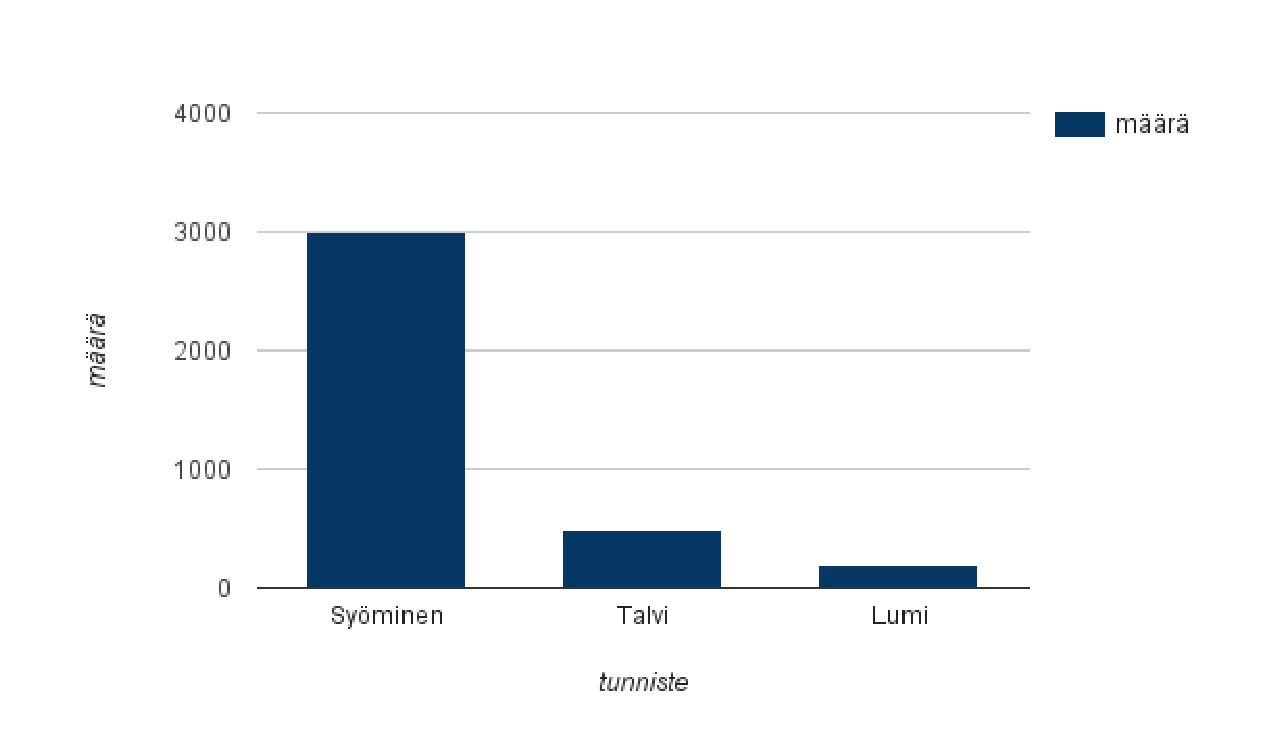
\includegraphics[width = 380pt]{tunnisteet.eps}\caption{Esimerkin tunnisteiden jakautuminen kuvitteellisessa datassa.}
\label{esimerkkitunnisteet}
\end{figure}
\begin{figure}[]
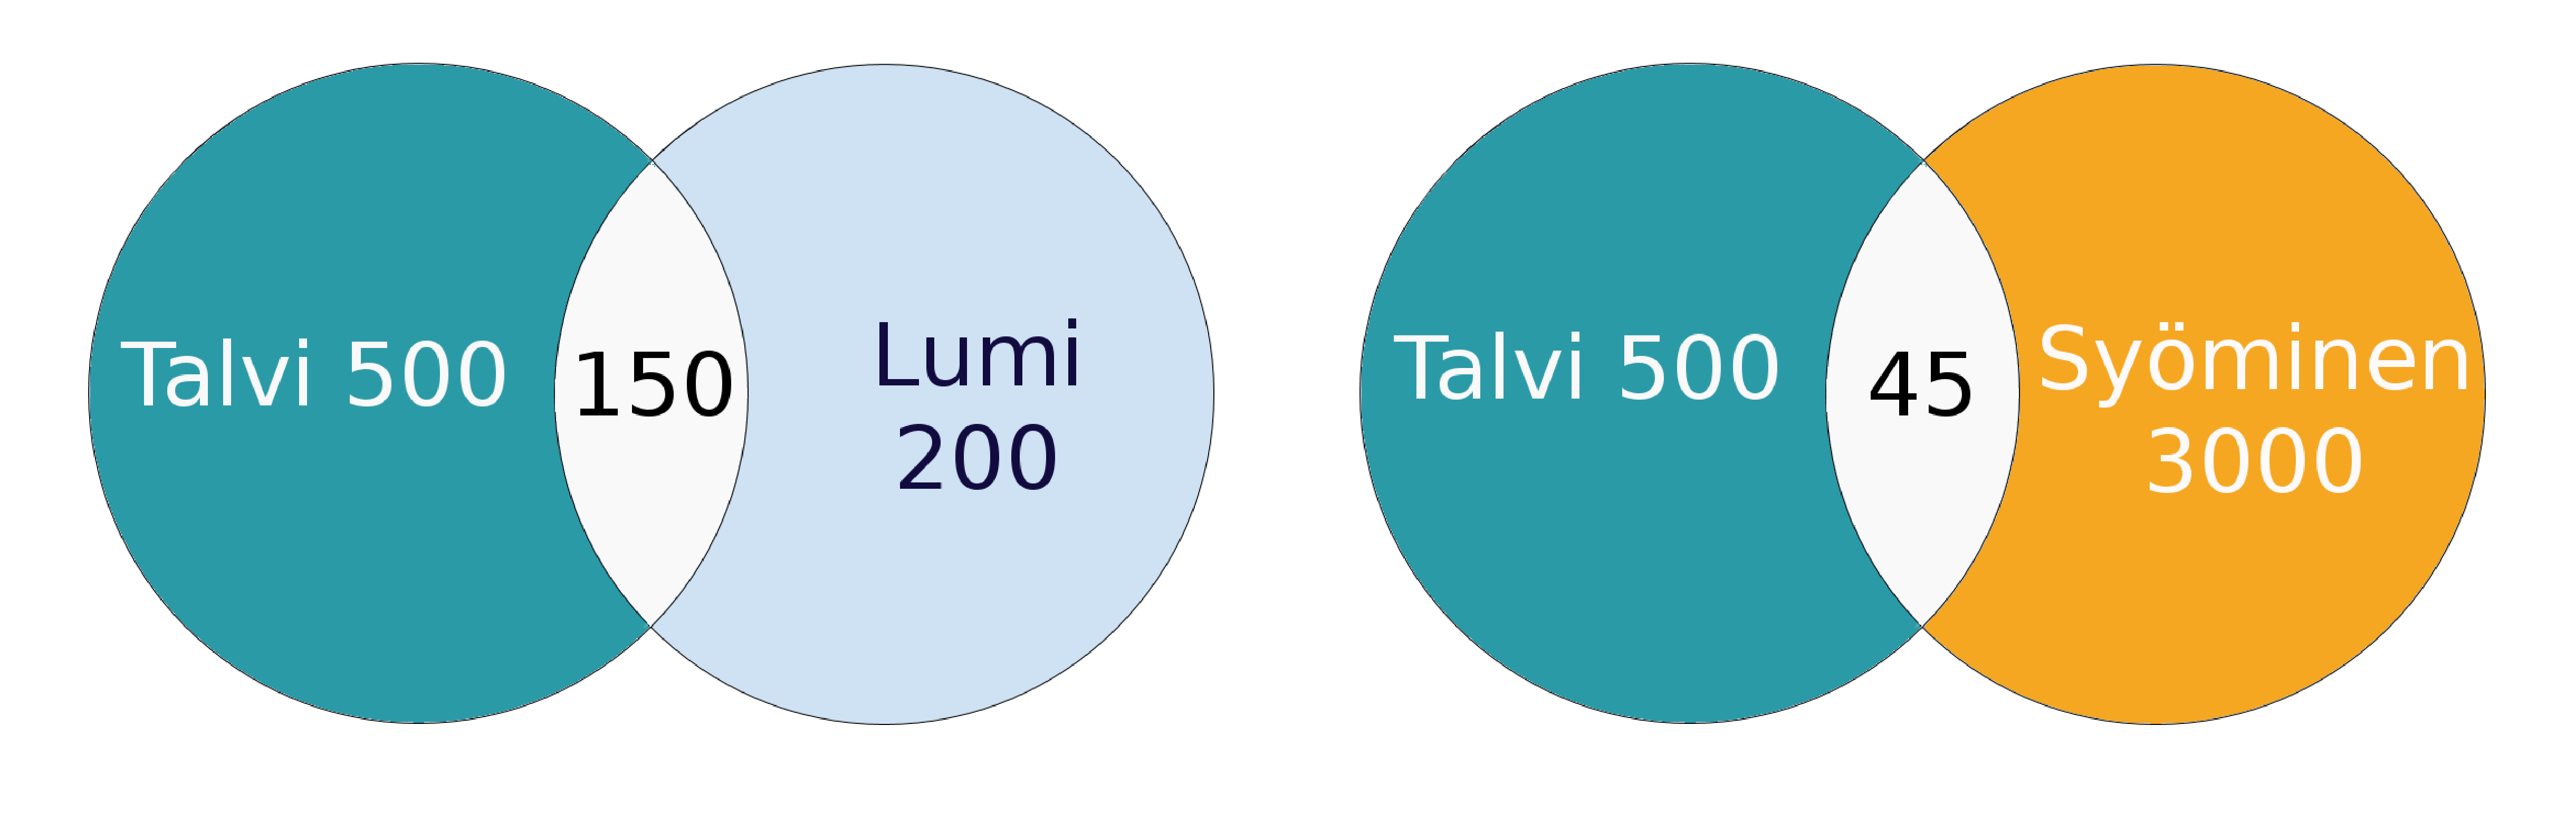
\includegraphics[width = 400pt]{vennit.eps}\caption{Tarkasteltavien tunnisteiden yhteisesiintyminen.}
\label{vennit}
\end{figure}
Havainnollistetaan seuraavaksi tunnisteiden suosittelua esimerkillä. Tarkastellaan kolmea eri tunnistetta, joiden osuus kaikista tunnisteista on merkitty kuvaan \ref{esimerkkitunnisteet}. Tarkasteltavat tunnisteet ovat \textit{Talvi}, \textit{Lumi} ja \textit{Syöminen}. Tarkastellaan tilannetta jossa käyttäjä merkitsee kuvansa tunnisteella \textit{Talvi}. Päätetään, että tunnisteet \textit{Talvi} ja \textit{Lumi} esiintyvät muissa kuvissa yhdessä 150 kertaa ja tunnisteet \textit{Talvi} ja \textit{Syöminen} 45. Tämä näkyy kuvassa \ref{vennit}. Vertaillaan ensin tunnisteiden \textit{Talvi} ja \textit{Lumi} yhteisesiintyvyyttä kaavalla 
\begin{displaymath} 
P (Lumi | Talvi):= \frac{|K(Talvi) \cap K(Lumi)|} {|K(Talvi)|}
\end{displaymath}
josta saadaan luku 0,3.
Tehdään sama tunnisteille \textit{Talvi} ja \textit{Syöminen} ja saadaan luku 0,09. 

Tunniste \textit{Lumi} sai korkeamman arvosanan, joten suosittelemme sitä käyttäjälle mieluummin kuin tunnistetta \textit{Syöminen}. Lumi vaikuttaa luontevammalta parilta talvelle kuin syöminen, joten tunnistesuosituksen voidaan sanoa olevan hyödyllinen. Oikeassa tapauksessa yhteisesiintyviä tunnisteita käyttäjän antamalle tunnisteelle olisi paljon enemmän kuin kaksi ja suositeltavien tunnisteiden listakin pitenisi.

Myös tarkasteltavassa artikkelissa todettiin edellä esitellyn suosittelustrategian tuottavan hyöviä tuloksia. \cite{Sigurbjornsson:2008:FTR:1367497.1367542}


\section{Yhteistoiminnallisen suodattamisen järjestelmät}
\subsection{Yleisesti}
        Yhteistoiminnalliseen suodattamiseen perustuvissa suosittelujärjestelmissä otetaan yksittäisen käyttäjän ja tuotteiden sijasta huomioon kaikkien käyttäjien väliset riippuvuudet. Suositusjärjestelmä vertaa käyttäjästä kerättyjä tietoja muiden käyttäjien tietoihin ja luokittelee käyttäjät samanlaisten mieltymysten perusteella pienemmiksi ryhmiksi. Jos joku tällaisen ryhmän jäsenistä on pitänyt jostakin tietystä tuotteesta, suositellaan tuotetta muillekin ryhmän jäsenille.
        
         Automaattisen yhteistoiminnallisen suodattamisen (ACF) järjestelmiä väitetään perinteisiä sisältöpohjaisia tehokkaammaksi, sillä tuotteiden suodattaminen pohjautuu koneanalyysin sijasta käyttäjäyhteisön relaatioihin~\cite{Herlocker:2000:ECF:358916.358995}. ACF-järjestelmät toimivat hyvin kaikenlaisen tiedon arvioinnissa, sellaisenkin, jota koneen on vaikea arvioita, kuten ihmisten makutottumukset tai laatuvaatimukset. ACF-järjestelmät eivät kuitenkaan ole syrjäyttäneet sisältöpohjaisia järjestelmiä, vaan niitä käytetään usein rinnakkain.
         
         Yhteistoiminnallisen suodattamisen järjestelmät voidaan jakaa vielä kahteen alatyyppiin: muistipohjaisiin ja mallipohjaisiin. Muistipohjaiset algoritmit tekevät ennusteita suoraviivaisesti käyttäjien arvosteluhistorioiden perusteella laskemalla eri käyttäjien tai tuotteiden samankaltaisuuksia. Yleisesti käytettäviä samankaltaisuuden mittaustapoja ovat Pearsonin korrelaatiokerroin ja kosinisamankaltaisuus (cosine similarity) arvosteluista muodostettujen vektoreiden välillä.
         
Mallipohjaiset algoritmit käyttävät historioita käyttäjien mallintamiseen ja ennustavat näillä malleilla tulevia arvosteluja kohteille, joita käyttäjät eivät ole vielä nähneet. Mallipohjaisia menetelmiä ovat esimerkiksi Bayesiläinen klusterointi, piilosemanttinen indeksointi (latent semantic indexing, LSI), todennäköisyyspohjainen piilosemanttinen indeksointi (PLSI) ja Markovin päätöksentekoprosessi (Markov Decision process) \cite{Das:2007:GNP:1242572.1242610}.
        
Yleinen tapa toteuttaa yhteistoiminnallisen suodattamisen suosittelujärjestelmä on käyttää muistipohjaisen ja mallipohjaisen tyypin yhdistelmää. Seuraavissa kappaleissa on esitelty kaksi eri projektia, jotka käyttivät kumpikin näiden tyyppien yhdistelmää.

\subsection{Netflix Prize -kilpailu}

        Suosittelujärjestelmät nousivat suuremman yleisön puheenaiheeksi digitaalisen elokuvavuokraamo Netflixin vuonna 2006 järjestämän Netflix Prize -kilpailun ansiosta. Kilpailun tarkoituksena oli parantaa Netflixin käyttämää suosittelujärjestelmää ja pienentää annetun testidatan keskineliöpoikkeamaa 10 prosentilla. Testidata koostui yli 100 miljoonasta elokuva-arvostelusta noin 480 000 käyttäjältä 17 770 eri elokuvasta. Bell ja Koren käsittelevät artikkelissaan ~\cite{Bell:2007:LNP:1345448.1345465} tässä kilpailussa vuoden sisällä parhaiten pärjänneen joukkueen suosittelujärjestelmämallia, joka saavutti 8,43 \%:n parannuksen.
        
        Huomattavaa joukkueen käyttämässä mallissa oli se, että se käytti kahden tärkeimmän yhteistoiminnallisen suodattamisen mallityypin yhdistelmää. Kummassakin mallissa on omat puutteensa, mutta yhdessä ne tuottivat hyviä tuloksia.
        
        Toinen näistä malleista on naapurustomalli (Neighborhood model, k-NN), joka on hyvä havaitsemaan paikallisia riippuvuuksia. Mallilla tarkastellaan kunkin alkion k:ta lähintä naapuria ja luokitellaan käsiteltävä alkio siihen ryhmään, jonka jäseniä on tarkasteltavissa naapureissa eniten. Kuvassa \ref{knn} on havainnollistettu naapurustomallin toimintaa. Mallilla koko tarkasteltava joukko saadaan jaettua pienempiin ryhmiin.
        
\begin{figure}[]
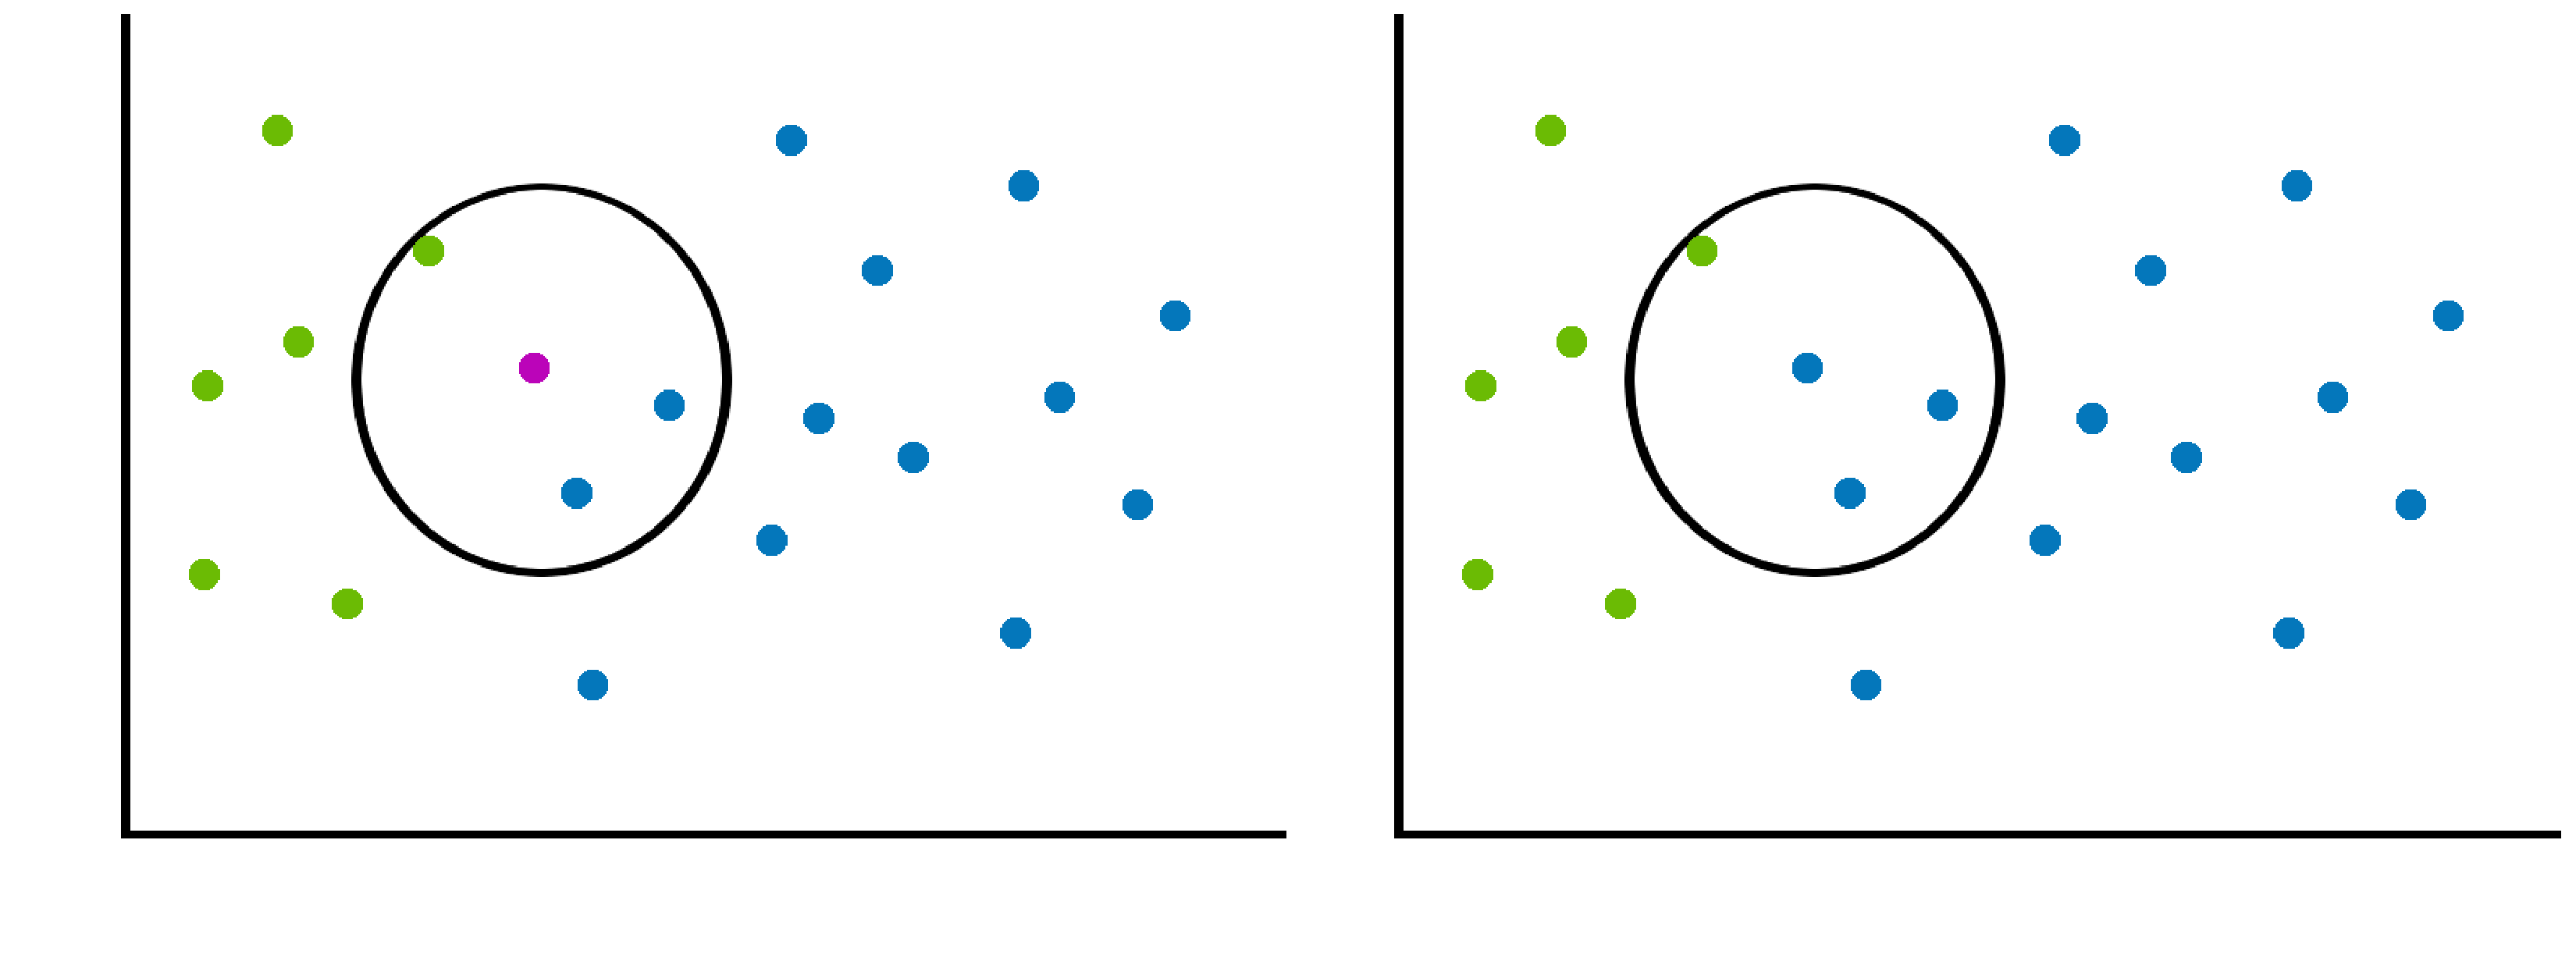
\includegraphics[width = 370pt]{knnkumpikin.eps}\caption{Naapurustomallin (k-NN) perusperiaate. Valitaan violetin yksilön k lähintä naapuria (tässä k = 3). Koska näissä naapureissa on enemmän sinisiä naapureita, luokitellaan violetti sinisten joukkoon.}
\label{knn}
\end{figure} 
 
Joukkueen käyttämässä naapurustomallissa elokuvat jaotellaan pareihin, jotka on arvosteltu pääsääntöisesti samalla tavalla. Näiden parien avulla pyritään ennustamaan käyttäjän mielipide elokuvasta, jota hän ei ole arvostellut. Naapurustomalli ottaa huomioon vain osan käyttäjän arvosteluista eikä siis havaitse niissä piileviä heikkoja signaaleja.

        Piilomuuttujamallit tulevat apuun siinä, missä naapurustomallissa on puutteita. Kun naapurustomalli havaitsee vain samankaltaisten elokuvien suhteet, hahmottaa piilomuuttujamalli elokuvien väliset riippuvuudet kattavammin. Se pystyy esimerkiksi havaitsemaan saman lajityypin elokuvien olevan samankaltaisia keskenään. Toisin kuin naapurustomallit, se ei kuitenkaan huomioi pieniä, keskenään samankaltaisista elokuvista muodostuvia ryhmiä. Malli ei esimerkiksi pysty suosittelemaan trilogian ensimmäisen osan katsoneelle käyttäjälle sarjan toista osaa. Joukkueen käyttämän piilomuuttujamallin toiminta perustuu käyttäjästä ja elokuvasta muodostettaviin vektoreihin, joiden avulla saadaan ennuste käyttäjän arviolle elokuvasta.
        
        \textit{joukkue käytti PARANNELTUA naapurustomallia, tänne MITEN he sitä paransivat ja miksi! tästä tarkemmin artikkelissa \cite{Koren:2008:FMN:1401890.1401944}}
        
        \textit{naapurustomallia ja piilomuuttujamallia käytettiin yhdistelmänä, tänne MITEN}
        
        Joukkue huomasi olevan oleellista katsoa dataa muutenkin kuin arvostelujen sisältöjen osalta. Laajemman kuvan saamiseksi joukkue keskittyi myös siihen, minkä tyyppisiä elokuvia käyttäjä ylipäätään vaivautuu arvostelemaan. Se, mikä elokuva on niin vaikuttava, että se kannattaa arvostella, opettaa paljon käyttäjästä. Jotkut mallit ottivat huomioon myös muun muassa arvostelujen määrän, keskiarvon ja päivämäärät.
        
Haasteetta projektille toi ihmisten elokuvamaun mallintamisen vaikeus. Mallinnuksessa tulisi ottaa huomioon muun muassa sellaisia piirteitä kun tietynlainen tunnelma, äänimaailma tai dialogin laadukkuus ja päätellä niistä käyttäjän elokuvamakua. Tällaisten ominaisuuksien huomioon ottaminen on kuitenkin algoritmisesti hyvin vaikeaa.
        
        Projektia vaikeuttivat myös käyttäjien vähäiset tai hajanaiset arviot testidatassa. Joukkue kehitti sekä naapurustomallia että piilomuuttujamallia tehokkaammaksi ja tarkoitukseen sopivammiksi. Eniten ongelmia tuotti datassa esiintyvä puutteellisuus arvojen osalta. Käytettävät mallit ovat standardimuodoltaan sellaisia, etteivät ne huomioi arvosteluiden vähäisyyttä. Jossakin tapauksessa olisi järkevämpää jättää jokin arvo kokonaan huomiotta kuin vääristää laskentaa puutteellisilla tiedoilla. Tästä aiheutuva ylisovittaminen (over fitting) oli yksi ongelma, jota saatiin vähennettyä parannetuilla malleilla.
        
Artikkelin julkaisemisen jälkeen Netflixin toimintaperiaate on muuttunut elokuvavuokraamosta suoratoistopalveluksi. Tämä vaikuttaa datan muotoon ja käyttäjien käyttäytymiseen. Myös suosittelujärjestelmien toimintaa on siksi muutettu edellä esitellyistä malleista. Artikkelissa ennakoitiin muutosta pohdinnassa, jossa esitettiin parempia suosittelutuloksia saatavan aikaiseksi seuraamalla itse arvostelujen ohella muita tietoja. Tällaisia ovat esimerkiksi käyttäjän selaus- tai hakuhistoria.~\cite{Bell:2007:LNP:1345448.1345465}

\subsection{Uutisartikkelien suosittelu käyttäjille - skaalautuva yhteistoiminnallinen suodattaminen}

\begin{figure}[]
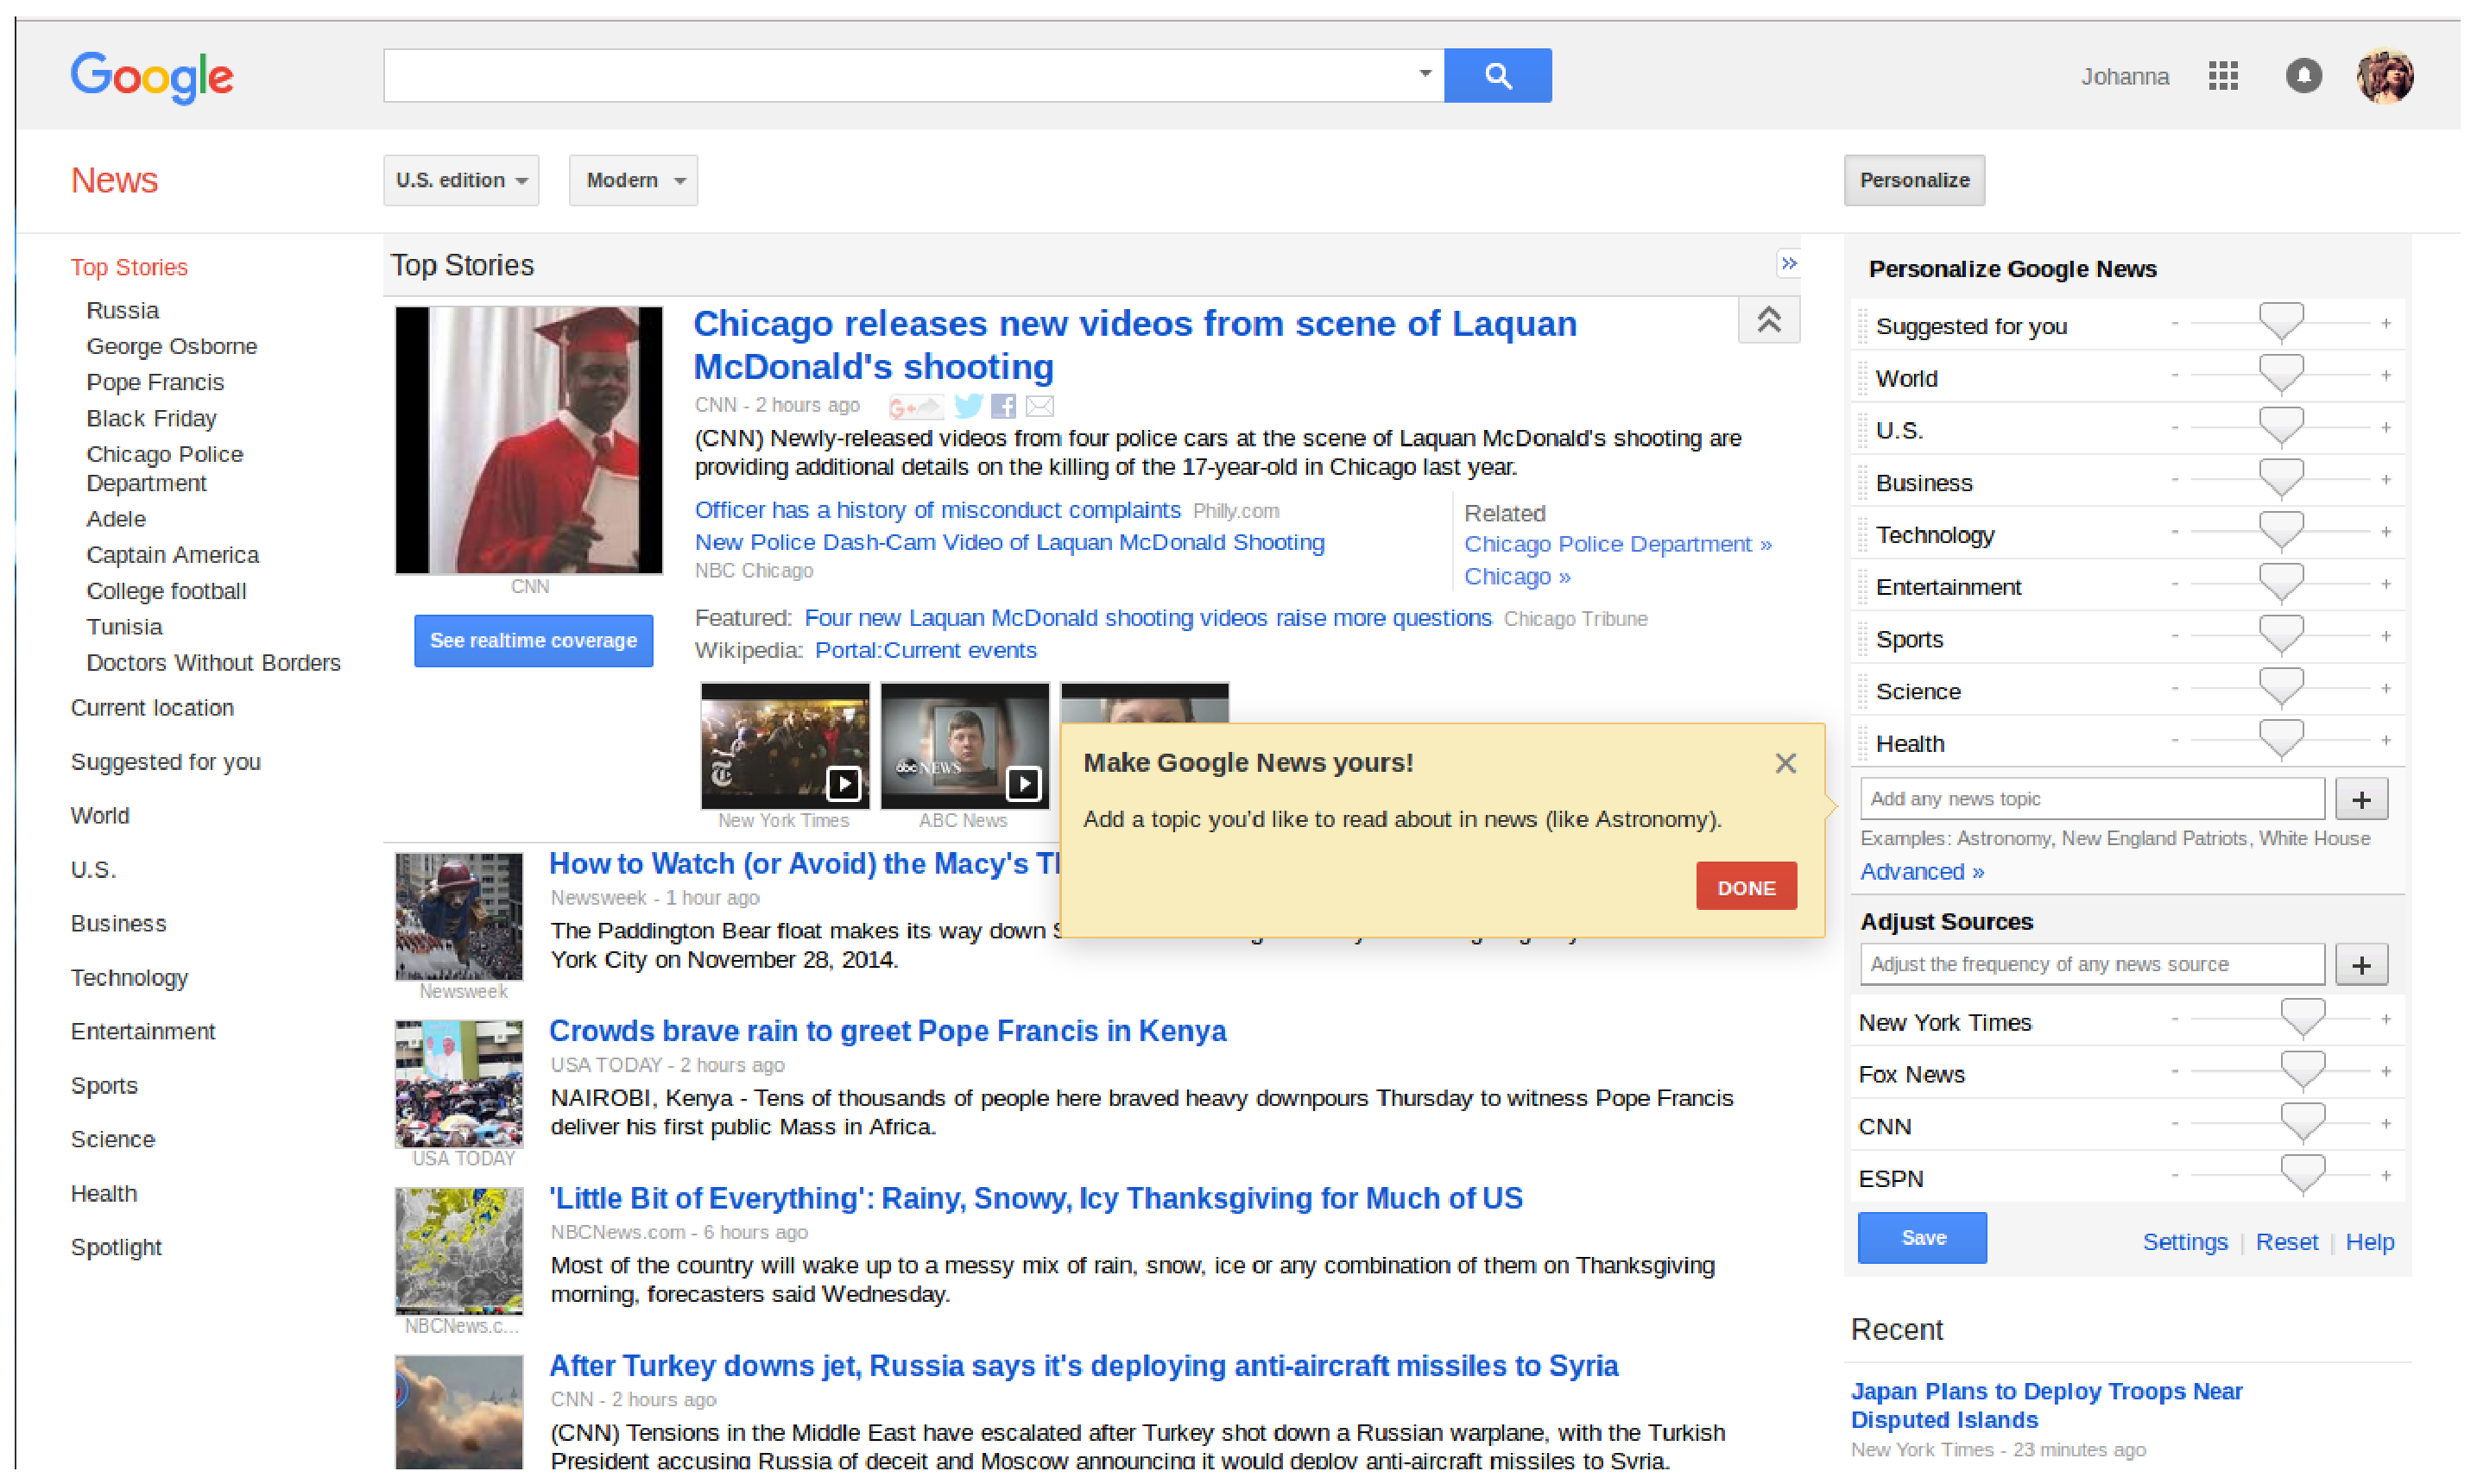
\includegraphics[width = 390pt]{googlenews.eps}\caption{Kuvankaappaus Google Newsistä.}
\label{googlenews}
\end{figure} 

Google News on palvelu, joka kokoaa käyttäjilleen uutisartikkeleita monelta eri uutissivustolta ja luokittelee keskenään samanlaiset artikkelit ryhmiin. Käyttäjille tarjotaan suosituksia luettavista artikkeleista heidän lukuhistoriansa perusteella. Das ym. \cite{Das:2007:GNP:1242572.1242610} esittelevät artikkelissaan yhteistoiminnalliseen suodattamiseen perustuvan ratkaisuehdotuksensa suosittelujen tarjoamiseen. Ryhmän päätavoitteenaan oli rakentaa skaalautuva online-suosittelujärjestelmä, jota voitaisiin käyttää suurissa palveluissa kuten Google Newsissä.

Google News -palvelun ominaisuudet loivat joitakin haasteita järjestelmän rakentamiselle. Valtava kävijämäärä ja miljoonat uutisartikkelit asettavat vaatimuksen skaalautuvuudelle. Palvelun osiot ovat myös jatkuvassa muutoksen tilassa, kun artikkeleita poistuu ja lisätään muutaman minuutin välein. Toisin kuin monissa muissa staattisissa palveluissa, käytettävä suosittelumalli vanhenee nopeasti eikä korjaannu pienillä muutoksilla. Osioiden jatkuva muutos on merkittävin tekijä, joka erottaa rakennettavan järjestelmän muiden suurien palveluiden suosittelujärjestelmistä \cite{Das:2007:GNP:1242572.1242610}.

Google News -palvelulla on käyttäjänä sekä rekisteröitymättömiä että rekisteröityneitä käyttäjiä, joista jälkimmäisille tarjotaan enemmän käytettäviä ominaisuuksia. Kuvassa \ref{googlenews} näkyy rekisteröityneen käyttäjän näkymä palvelussa. Käyttäjän niin salliessa Google tallentaa rekisteröityneen käyttäjän uutisartikkeleihin liittyviä aktiviteetteja muiltakin Googlen palveluilta ja tallentaa nämä artikkelit käyttäjän lukuhistoriaan Google News -palvelussa. Esimerkki tällaisesta aktiviteetista voisi olla vaikka uutisartikkelin hakeminen Googlen hakukoneella. Kootun historian pohjalta muodostetaan artikkelisuosituksia, joista kolmea tarjotaan käyttäjän luettavaksi. Artikkelin projektissa keskityttiin suosituksien antamiseen juurikin rekisteröityneille käyttäjille. 

Toisin kuin joissakin suositusjärjestelmiä käyttävissä palveluissa, Google Newsissä tarkasteltavat tuotteet eivät saa suoraa arvosanaa käyttäjältään. Projektissa päätettiinkin käsitellä käyttäjän käyttäytymistä arvioinnin pohjana siten, että klikkaus uutisartikkeliin tulkitaan myönteisenä äänenä artikkelille. Päätöstä perusteltiin sillä, että käyttäjille tarjotaan lyhyt, selkeä kuvaus jokaisesta artikkelista listausnäkymässä. Voidaan siis olettaa, että käyttäjä on todennäköisimmin kiinnostunut artikkelista, jos hän vielä kuvauskappaleen lukemisenkin jälkeen päättää klikata artikkelia. Klikkaukset kuvastavat kuitenkin vain käyttäjien myönteisiä mielipiteitä, eivätkä kerro mitään siitä, mistä käyttäjät eivät pidä \cite{Das:2007:GNP:1242572.1242610}.

Google News -palvelu on yksi maailman suosituimmista uutissivustoista. Tarkasteltavassa projektissa havainnoitiin uutisartikkeleita yhden kuukauden ajalta ja artikkeleita kertyi useita miljoonia. Käyttäjien klikkausaktiivisuus artikkeleihin on hyvin vaihtelevaa ja klikkaushistorioiden koko vaihtelee nollasta satoihin tai jopa tuhansiin.

Google asettaa tarkkoja vaatimuksia palveluidensa vasteajoille myös Google Newsin kohdalla. Esimerkiksi kotisivun näkymä generoidaan tyypillisesti sekunnissa. Tästä sekunnista jää muiden toimintojen jälkeen jäljelle muutama sata millisekuntia suositteluiden muodostamiseen. Tiukat aikavaatimukset olivatkin yksi projektin haasteista.

Kappaleessa 3.1 esiteltiin jako malli- ja muistipohjaisiin yhteistoiminnallisen suodattamisen järjestelmiin. Artikkelissa käsiteltävässä järjestelmässä käytettiin niin sanottua hybridimallia, eli sekoitusta kummankin tyyppisestä järjestelmästä.

Muistipohjaisena algoritmina toimii Covisitation, jota esitellään tarkemmin jäljempänä. Mallipohjaisessa lähestymisessä käytetään kahta klusterointitekniikkaa, algoritmeja PLSI (probabilistic latent semantic indexing) ja MinHash. Kaikki nämä kolme algoritmia asettavat tarkasteltaville uutisartikkeleille arvosanat siten, että paremmat suositukset saavat korkeamman numeerisen arvon. Lopussa kaikki kolme arvosanaa yhdistetään painottaen kaavalla
\begin{displaymath}
\sum_a{w_a r^{(a)}_{s}}
\end{displaymath}
missä $w_a$ on algoritmin $a$ paino ja $r^{(a)}_{s}$ on algoritmin $a$ antama arvosana artikkelille $s$ ja saadaan järjestetty lista artikkeleita. Tästä listasta valitaan K parhaimman arvosanan saanutta artikkelia ja suositellaan niitä käyttäjälle.

Ensimmäisenä esittelemme todennäköisyyspohjaisen klusterointialgortimin MinHash. MinHash jakaa parin käyttäjiä samaan klusteriin sen todennäköisyyden perusteella, jolla käyttäjät ovat äänestäneet eli klikanneet samoja artikkeleita. Jokainen käyttäjä $u \in U$ esitetään tämän klikkaushistoriana $C_u$, eli joukkona artikkeleita, joita kyseinen käyttäjä on klikannut.

Kahden käyttäjän $u_i$ ja $u_j$ samankaltaisuus on mahdollista mitata käyttämällä jo kappaleessa 2.2 esiteltyä Jaccardin kerrointa $S(u_i, u_j) = \frac{|C_{u_{i}} \cap C_{u_{j}}|}{|C_{u_{i}} \cup C_{u_{j}}|}$. Jos haluaisimme tarjota käyttäjälle $u_i$ suosittelua, laskisimme ensin tämän samankaltaisuuden kaikkien muiden käyttäjien $u_j$ kanssa ja suosittelisimme sitten (käyttäjälle $u_i$) muiden käyttäjien $u_j$ äänestämiä artikkeleita, joiden paino on yhtäläinen suureen $S(u_i, u_j)$ kanssa. Tämän tekeminen reaaliajassa ei kuitenkaan ole skaalautuvaa, joten Jaccardin kerroin ei semmoisenaan kelpaa artikkelin projektin käyttöön.

Ongelman ratkaisuna käytetään tiivisteiden muodostamista LSH-tekniikalla. LSH:n keskeinen ajatus on muodostaa datapisteistä tiiviste useita tiivistefunktioita käyttäen ja päätellä läheiset naapurit kyselypisteen tiivisteen avulla. Jaccardin kertoimen kanssa käytettäväksi soveltuu LSH-tekniikka MinHash. MinHashin perusidea on permutoida satunnainen joukko artikkeleita ($S$) ja laskea jokaiselle käyttäjälle $u_i$ tiivistearvo indeksinään ensimmäinen artikkeli permutaatiossa, joka kuuluu käyttäjän artikkelijoukkoon $C_{u_{i}}$. Todennäköisyys, että kahdella kaikkien $S$:n permutaatioiden joukosta valitulla permutaatiolla on sama tiiviste, on täysin yhtenevä  niiden Jaccardin kerroin -luvun eli samanlaisuuden kanssa. MinHashin jokaisen tiivisteämpärin (hei nyt... hash bucket, miten se oikein käännetään?) voidaan ajatella vastaavan klusteria. Samaan klusteriin laitetaan kaksi käyttäjää todennäköisyydellä, joka on yhtenevä näiden käyttäjien artikkelijoukkojen samankaltaisuudella $S(u_i, i_j)$.

Toinen esitelty klusterointialgoritmi PLSI mallintaa käyttäjät ($u \in U$) ja artikkelit ($s \in S$) satunnaismuuttujina.
Käyttäjien ja artikkeleiden väliset suhteet opitaan mallintamalla yhteisjakauma käyttäjistä ja artikkeleista sekoitejakaumana (mixture distribution).
Suhdetta merkitään piilomuuttujalla Z, jonka voidaan ajatella kuvastavan käyttäjä- ja artikkeliyhteisöjä siten, että samankaltaiset käyttäjät ovat oma yhteisönsä ja samankaltaiset artikkelit omansa. Malli voidaan kirjoittaa sekoitemallina
\begin{displaymath}
p(s|u;0)= \sum_{z=1}^{L} {p(z|u)}{p(s|z)}
\end{displaymath}
kun $Z$ saa arvoja väliltä $z \in Z$ ja $||Z|| = L$.

Covisitation(tälle tarttee ehkä suomennoksen) esiteltiin projektin muistipohjaisena osiona. Covisitation on tapahtuma, jossa sama käyttäjä klikkaa kahta artikkelia tietyn ajan sisällä. Voimme ajatella uutisartikkeleita verkkona, jossa artikkelisolmut on painotettu covisitation-lukumäärillä.   
\textit{pitäisikö olla pieni kuva tällaisesta painotetusta verkosta...}
Tätä verkkoa käsitellään vierekkäisyyslistana Bigtablessa, jonka avaimina on artikkeli-id:t.
Kun havaitaan käyttäjän $u_i$ klikkaavan artikkelia $s_k$, käydään läpi kyseisen käyttäjän klikkaushistoria $C_{u_{i}}$. Jokaisen artikkelin $s_k \in C_{u_{i}}$ kohdalla muokataan sekä $s_j$ ja $s_k$ vierekkäisyyslistoja lisäämällä niihin kyseiseen klikkaukseen viittaava uusi merkintä. Jos kyseiselle parille on jo olemassa merkintä, päivitetään age discounted count(iih suomennos tälle).

\section{Pohdinta}
Ehkäpä täällä voisi olla vaikka kappalekohtaista pohdintaa. Esim jotain tägeistä, jotain ihmisten elokuvamausta jne. Ja sitten jotain yleistä, jos jotain keksii... Ehkä, tai sitten koko pohdinta pois.

        
\section{Yhteenveto}

Suosittelujärjestelmiä tarvitaan monessa eri kontekstissa. Esimerkkini sisältöpohjaisen suodattamisen suosittelujärjestelmästä on hyvälaatuisten tunnisteiden suosittelu käyttäjille. Tässä tulee esille ikään kuin kahden kerroksen suosittelua. Ensin käyttäjille suositellaan tunnisteita, jotka sopivat heidän kuviinsa. Näitä hyviä tunnisteita käyttämällä mahdollistuu toinen suositteluominaisuus, eli kuvien suositteleminen niitä selaaville käyttäjille. Palvelu voi suositella käyttäjille heitä kiinnostavia kuvia käyttämällä joko sisältöpohjaista tai yhteistoiminnallista suosittelujärjestelmää.

Sisältöpohjaisen ja yhteistoiminnallisen suosittelujärjestelmän ero on pohjimmiltaan siinä, käytetäänkö suositteluun vain yhden käyttäjän vai koko käyttäjäyhteisön mieltymyksiä. Tehokkaimmat tulokset näytettäisiin saavan käyttämällä useamman kuin yhden suosittelumallin yhdistelmää ~\cite{Bell:2007:LNP:1345448.1345465}.





% -akoskdoasjfoasf-- References ---
%
% bibtex is used to generate the bibliography. The babplain style
% will generate numeric references (e.g. [1]) appropriate for theoretical
% computer science. If you need alphanumeric references (e.g [Tur90]), use
%
% \bibliographystyle{babalpha-lf}
%
% instead.

\bibliographystyle{babplain-lf}
\bibliography{references-fi}


% --- Appendices ---

% uncomment the following

% \newpage
% \appendix
 
% \section{esimerkki}

\end{document}
